%%%%% rvsi
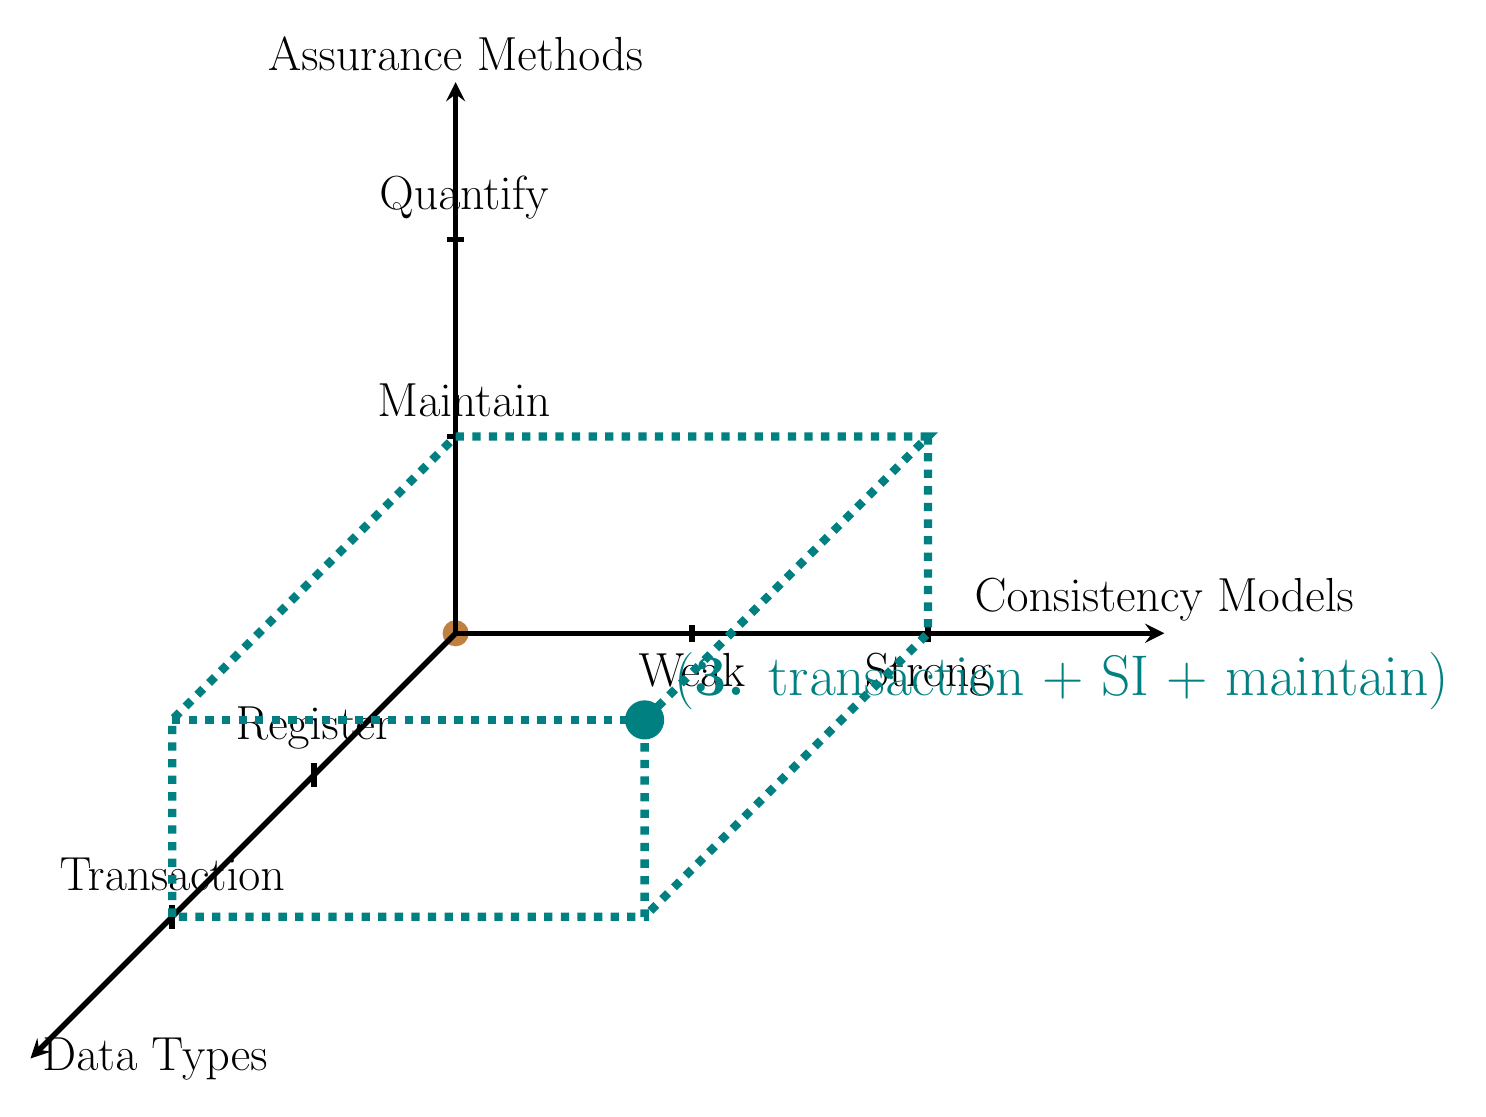
\begin{tikzpicture}[x = 0.5cm, y = 0.5cm, z = 0.3cm, >=stealth, font = \LARGE]

\begin{scope}[axesfont/.style = {font = \LARGE}, axesline/.style = {->, line width = 2}, 
  tickline/.style = {line width = 2}, tickfont/.style = {font = \LARGE}]

% the origin
\node[fill = brown, circle] at (0,0,0) {};
% The axes
\draw[axesline] (xyz cs:x=0) -- (xyz cs:x = 18) node[above, axesfont] {$\textrm{Consistency Models}$};
\draw[axesline] (xyz cs:y=0) -- (xyz cs:y = 14) node[above, axesfont] {$\textrm{Assurance Methods}$};
\draw[axesline] (xyz cs:z=0) -- (xyz cs:z = -18) node[right, axesfont] {$\textrm{Data Types}$};

% The ticks

% ticks for consistency models
\draw[tickline] (6,-3pt) -- (6,3pt) node[below = 6pt, tickfont] {Weak};
\draw[tickline] (12,-3pt) -- (12,3pt) node[below = 6pt, tickfont] {Strong};

% ticks for assurance methods
\draw[tickline] (-3pt,5) -- (3pt,5) node[above = 3pt, tickfont] {Maintain};
\draw[tickline] (-3pt,10) -- (3pt,10) node[above = 3pt, tickfont] {Quantify};

% ticks for data types
\draw[tickline] (xyz cs:y=-0.3pt,z=-6) -- (xyz cs:y=0.3pt,z=-6) node[above = 1pt, tickfont] {Register};
\draw[tickline] (xyz cs:y=-0.3pt,z=-12) -- (xyz cs:y=0.3pt,z=-12) node[above = 1pt, tickfont] {Transaction};
\end{scope}

%%%%%%%%%% for RVSI
  \begin{scope}[line/.style = {dashed, line width = 3, teal}]
      \draw[line]
      (xyz cs:z=-12) coordinate (z) --
      (xyz cs:y=5, z=-12) coordinate (yz) --
      (xyz cs:y=5) coordinate (y) --
      (xyz cs:x=12, y=5) coordinate (xy) --
      (xyz cs:x=12, y=5, z=-12) coordinate (xyz) --
      (xyz cs:x=12, z=-12) coordinate (xz) -- cycle;

      \path[draw, line] (xy) to (xyz cs:x=12) coordinate (x) to (xz);
      \draw[line] (yz) to (xyz);

      \node (rvsi-maintain) [fill = teal, circle, inner sep = 5pt, label = {[above right, teal, font
      = \huge] 0: (\textbf{3.} transaction + SI + maintain)}] at (xyz) {};
	\end{scope}
\end{tikzpicture}
